\documentclass[]{article}
\usepackage{natbib}
\bibliographystyle{unsrtnat}
\usepackage{graphicx}
%\usepackage{placeins}
\usepackage[british]{babel}
\usepackage[autostyle]{csquotes}
\usepackage{url}
\DeclareGraphicsExtensions{.pdf,.png,.jpeg,.jpg}
\graphicspath{{images/}}
%\graphicspath{ {./images/} }
\usepackage{wrapfig}
\renewcommand{\figurename}{Fig.}
%opening

\title{Identifying macro-moths with micro-features}
\author{Paul J. Palmer}

\begin{document}

\maketitle

\begin{abstract}

This article explores the use of external microscopic characters to support the identification (ID) of  macro-lepidoptera. The usual process of identifying macro-moths  focusses on the wings, which are often large and distinctively patterned. Matching an unknown specimen to reference images is often the identification method employed, but when the wings are worn and the markings atypical matching patterns is fraught with difficulty.
 However, microscopic features, which are often overlooked with macro-moths, may be used to narrow the field of candidate taxa to arrive at a robust identification. 

\end{abstract}

\section*{A Difficult Specimen to ID}
The specimen used as an example here was taken at sugar 2020-08-16 on the Rutland Water Nature Reserve. It would have been recorded as a very worn example of \textit{Hypena proboscidalis} (The Snout) if it had not briefly raised its wings in a posture uncharacteristic for this species, placing an element of doubt in this presumed ID. As can be seen in Figure~\ref{fig:202009131026pjp-1}, the specimen lacks the long, forward pointing palps that give the Snout its vernacular name, buts its wings have the same slightly hooked shape  and it displays a similar median fascia as in the verified \textit{Hypena proboscidalis} illustrated in  Figure~\ref{fig:S202012271446-1}.  It would be easy to presume that the palps have been broken in what appears to be a worn specimen due to the ill-defined markings, but examination under magnification, as shown in  Figure~\ref{fig:20201112-1} reveals that the palps are short but undamaged. Less obvious,  is the lack of ocelli above the compound eye, clearly seen in Figure~\ref{fig:S202012271446-4}, which  eliminates \textit{Hypena proboscidalis} as a candidate taxon for the specimen.

\section*{The Identification Method}
Identification of an unknown Lepidoptera specimen may be thought of as the process by which the  observable features are matched to those of a known taxon.
For a general discussion on the topic of identification \citet{Pankhurst1978} is still relevant to the field naturalist today.
 Given that there are about 2,500 UK Lepidoptera taxa of which around 450 are thought of as \enquote{the larger moths} a systematic approach is needed as an alternative to randomly flipping through the pages of a guide looking for a match.
 
 Inspired by Pankhurst, the approach followed by the author is to list plausible candidate species and to mark each with a \enquote{+} for matching features and \enquote{-} contradicting features. A \enquote{?} is used to  indicates that a feature is either. \enquote{not known} or not yet determined. An identification is achieved when one of the candidates has multiple \enquote{+} and no \enquote{-} against its name.
 A well written dichotomous key will lead you through a functionally identical process, as will a computer driven \enquote{multi-access} key. Unfortunately, there are not many keys covering macro-moths such as those under consideration here.
 The take-away message is that a robust identification should always rely on the matching and rejection of multiple characters, not just wing pattern, and that some features  may be too small to be observed by the unaided eye.  
 
 In practical terms,  examination of specimens under  3 --- 30 x magnification reveals additional characters  in both live and preserved specimens that are useful for ID purposes. The low magnification required places these features in range of hand lenses and USB microscopes, and while good lighting is necessary, there is no need to specially prepare the specimen.

\section*{Making a Determination}
We start by noting observation about the unknown specimen:
Forewing length: 16.7 mm; Forewing width: 11.4, mm;  Ocelli: Absent;  Labial palps: Forward. Flight time: August. The gender can be determined by examination of the frenulum, which links the wings together in moths. In males, it consists of a single bristle in males, and a pair in females. Both specimens here are females.

Unfortunately there a few resources listing the features we need to consider, but a good place to start is the matrix key published by \citet{Dombroskie2011}. While it is intended for Canadian Lepidoptera, it can also be used to provide an indicative guide to UK lepidoptera families. Importantly, it is a useful indication of charactera that can be used to find the likely family of a specimen.

%In this case, although the specimen is a macro-moth, the family \textit{Erebidae}.
Using the Canadian Lepidoptera Key , (See Figure~\ref{fig:20201112-1}), the lack of oceli (simple eyes), coiled unscaled proboscis, and forward facing palps are suggestive of family \textit{Geometridae}. The forewing length of 16.7 mm and the flight time of August are also useful for eliminating many possible UK taxa.

A list of candidate \textit{Geometridae} based on size and general appearance can be made using  \citet{Skinner1984} or \citet{Waring2018}. A single species, \textit{Scotopteryx chenopodiata} (Shaded Broad-Bar),  matches the size and wingshape,  but the unidentified specimen appearance is very plain,  and lacks the median dark cross band usually considered typical. The text in Skinner notes the superficial resemblance of this species to \textit{Hypena proboscidalis}. The online resource at \url{http://www.lepiforum.de/lepiwiki.pl?Scotopteryx_Chenopodiata} has a photograph of a specimen also lacking the median dark cross band, confirming that such forms have previously been observed.

At this point we can be certain that we have arrived at a robust identification, so further investigation is not strictly necessary. However, 
the dissection in Figure~\ref{fig:202009131026pjp-3}  confirms \textit{Scotopteryx chenopodiata} when compared to the example at \url{http://www.lepiforum.de/lepiwiki.pl?Scotopteryx_Chenopodiata}.

\section*{Conclusions}
This example involving the correct separation of two common species of moth with superficial resemblance can easily be achieved with observations made at low magnifications. In this case the unusually plain form of the unknown specimen was instrumental in misdirection of the ID, a problem exacerbated by reliance on wing markings as the primary focus for identification.
%Using low power magnification allowed the use of microscopic characters to achieve a correct determination. This leads to the surprising conclusion that the ID process
We are led to the surprising conclusion that microscopic features in macro-lepidoptera are an overlooked character when achieving a correct determination.


\begin{figure}
	\centering
	\begin{minipage}{0.45\textwidth}
		\centering
	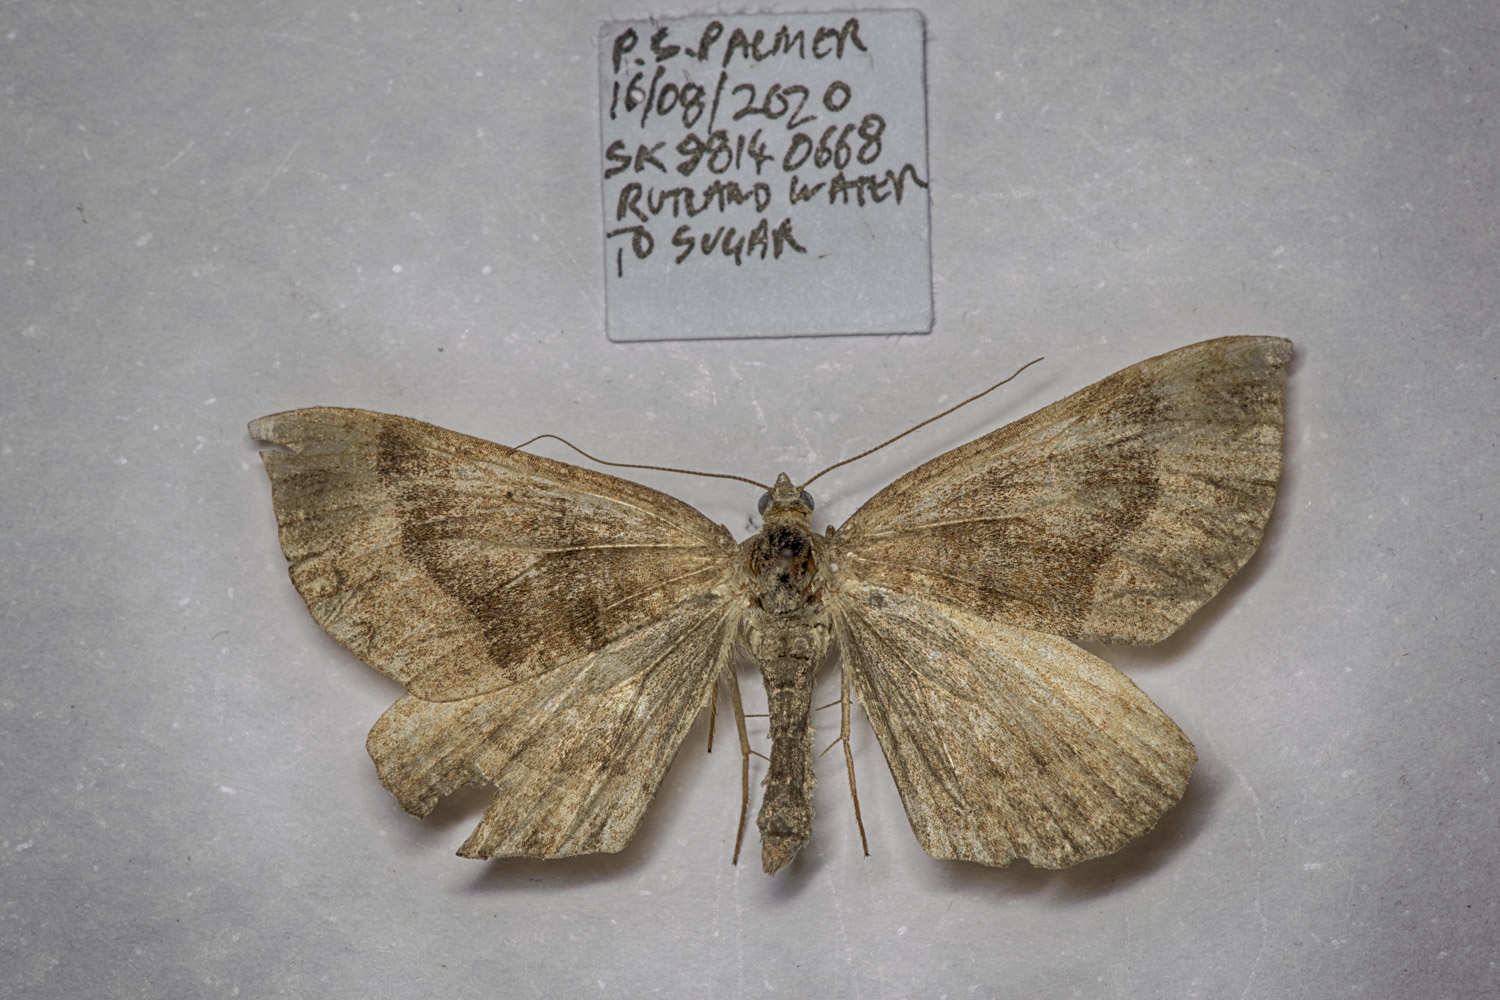
\includegraphics[width=0.9\linewidth]{202009131026PJP-1}
	\caption{The unkown specimen resembling Hypena proboscidalis.}
	\label{fig:202009131026pjp-1}
	\end{minipage}\hfill
	\begin{minipage}{0.45\textwidth}
		\centering
		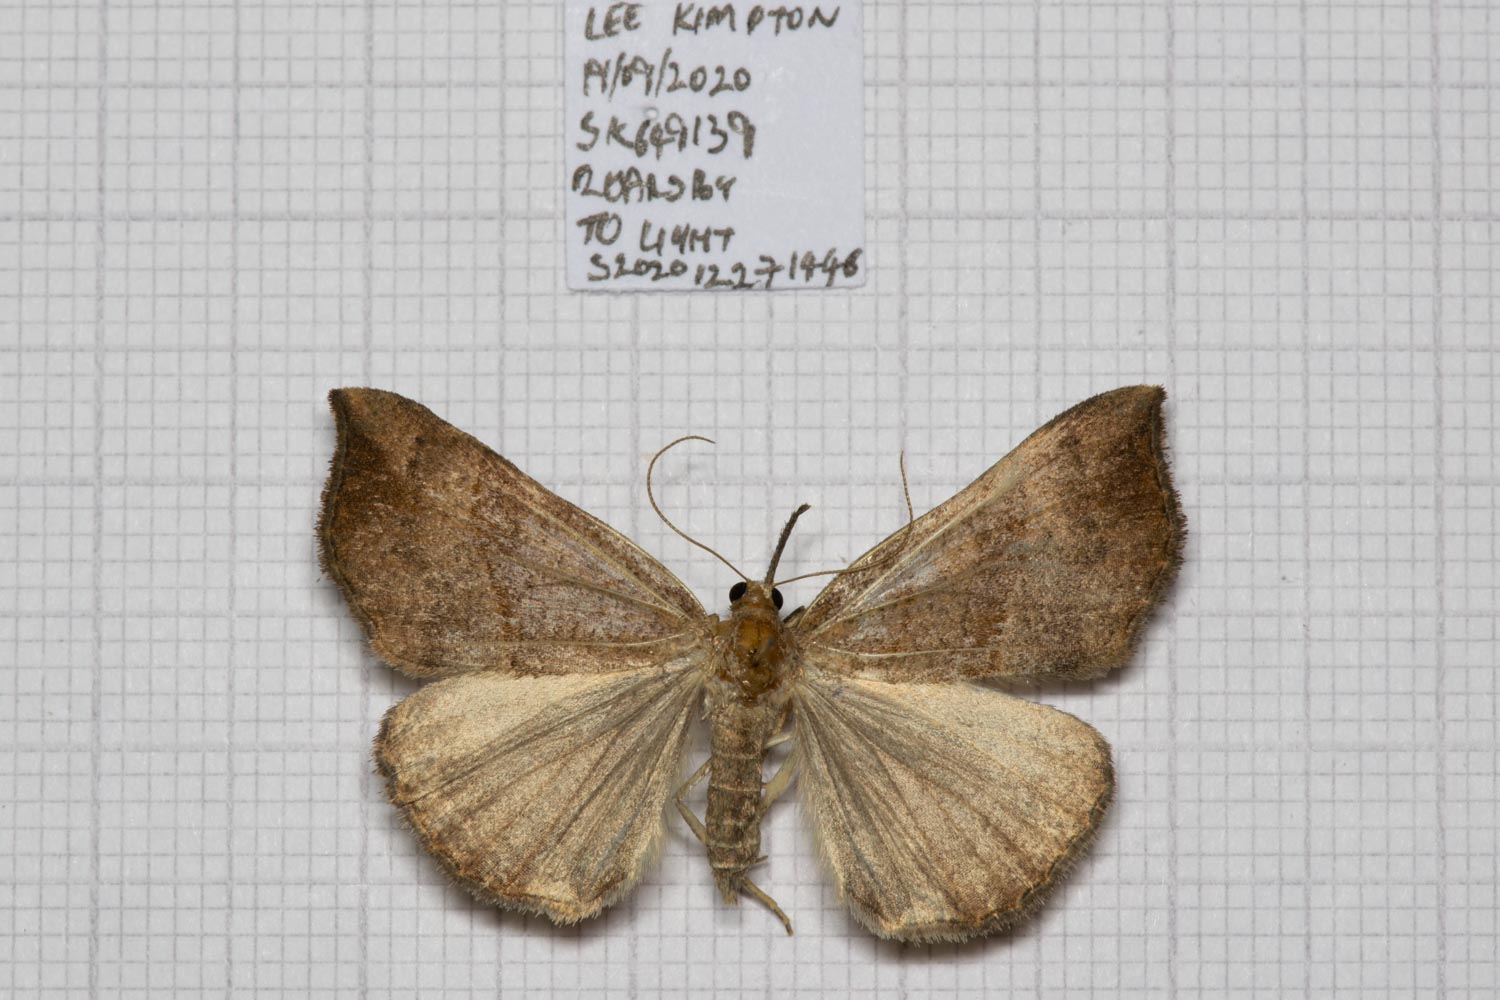
\includegraphics[width=0.9\textwidth]{S202012271446-1} % second figure itself
		\caption{A verified specimen of female Hypena proboscidalis.}
		\label{fig:S202012271446-1}
	\end{minipage}
\end{figure}



\begin{figure}
	\centering
	\begin{minipage}{0.45\textwidth}
		\centering
	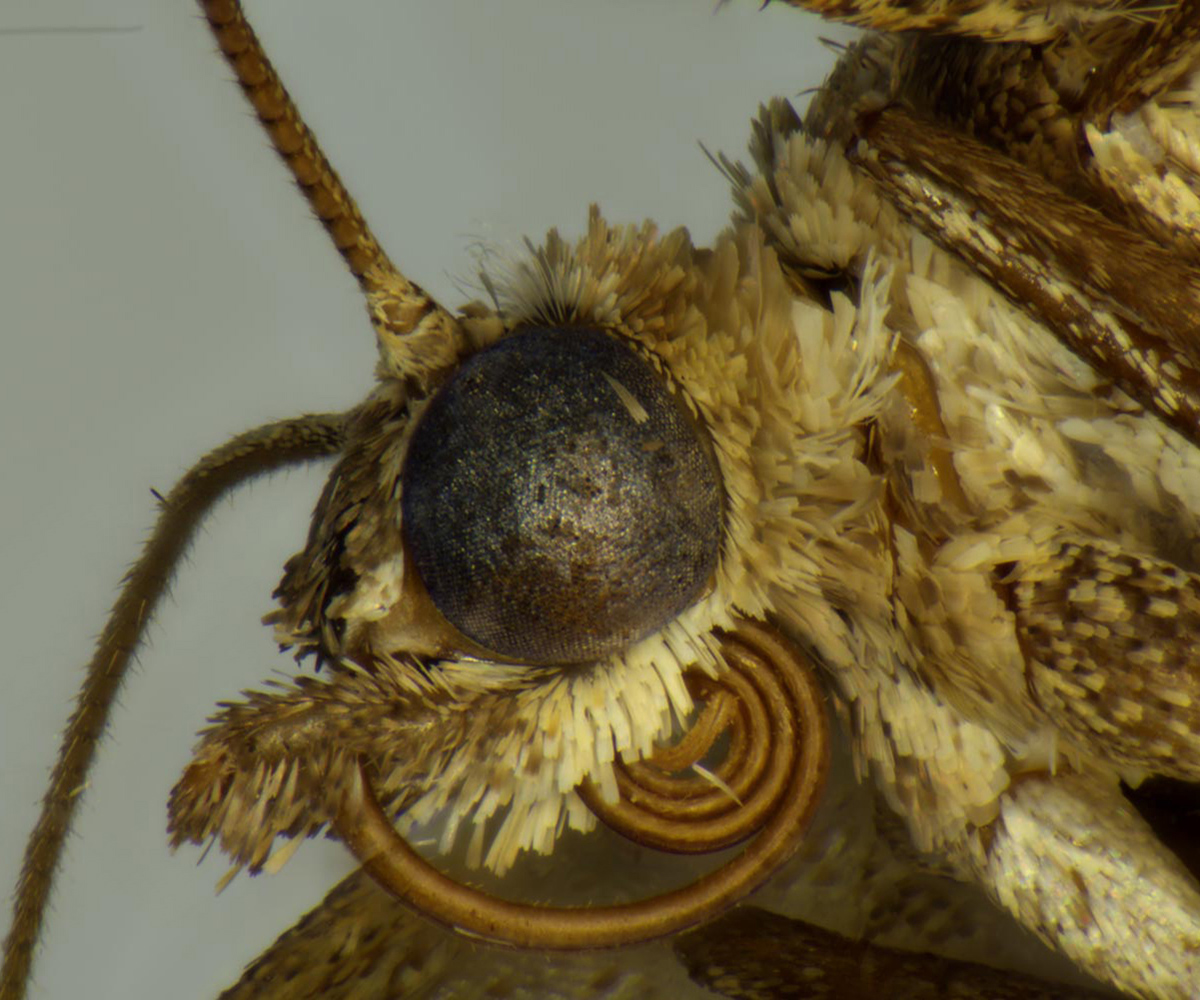
\includegraphics[width=0.9\linewidth]{202009131026PJP-4}
	\caption{Short undamaged palps eliminate Hypena proboscidalis as a candidate taxon.}
	\label{fig:20201112-1}
	\end{minipage}\hfill
	\begin{minipage}{0.45\textwidth}
		\centering
		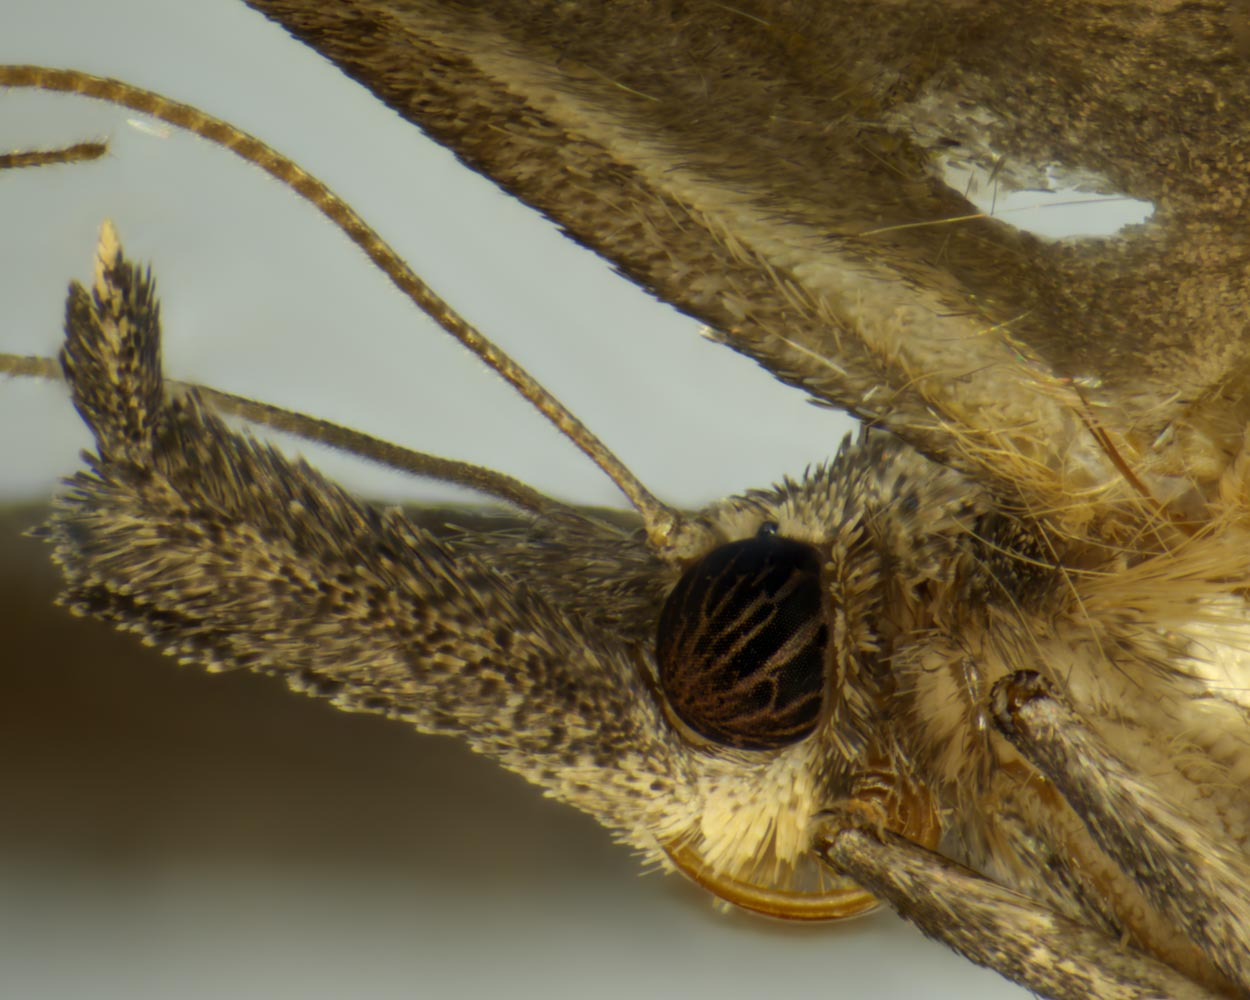
\includegraphics[width=0.9\textwidth]{S202012271446-4} % second figure itself
		\caption{Long, forward facing palps, and oceli above the compound eye of Hypena proboscidalis.}
		\label{fig:S202012271446-4}
	\end{minipage}
\end{figure}

\begin{figure}
	\centering
	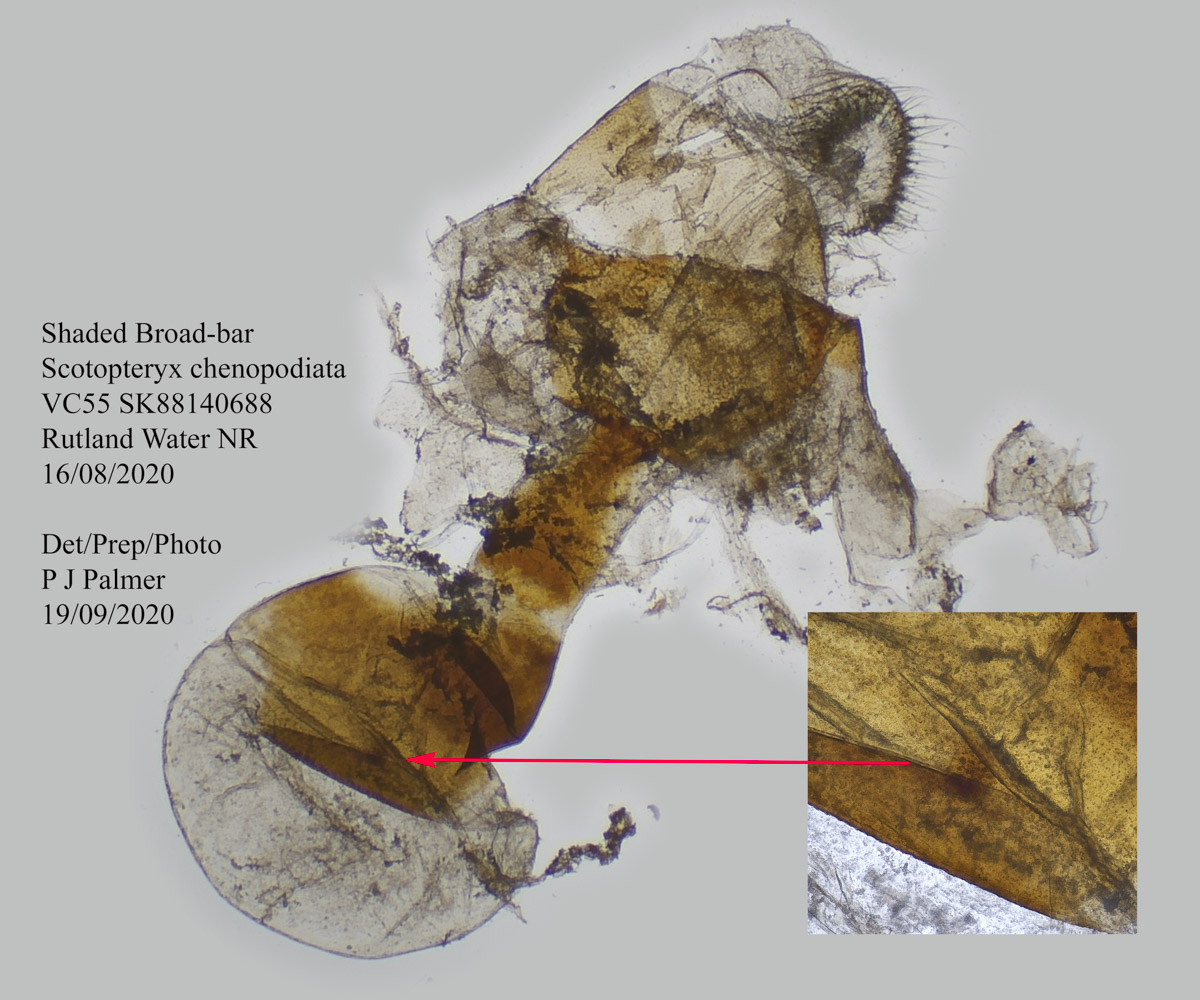
\includegraphics[width=0.7\linewidth]{202009131026PJP-3}
	\caption{Dissection}
	\label{fig:202009131026pjp-3}
\end{figure}


%
%\begin{figure}
%	\centering
%	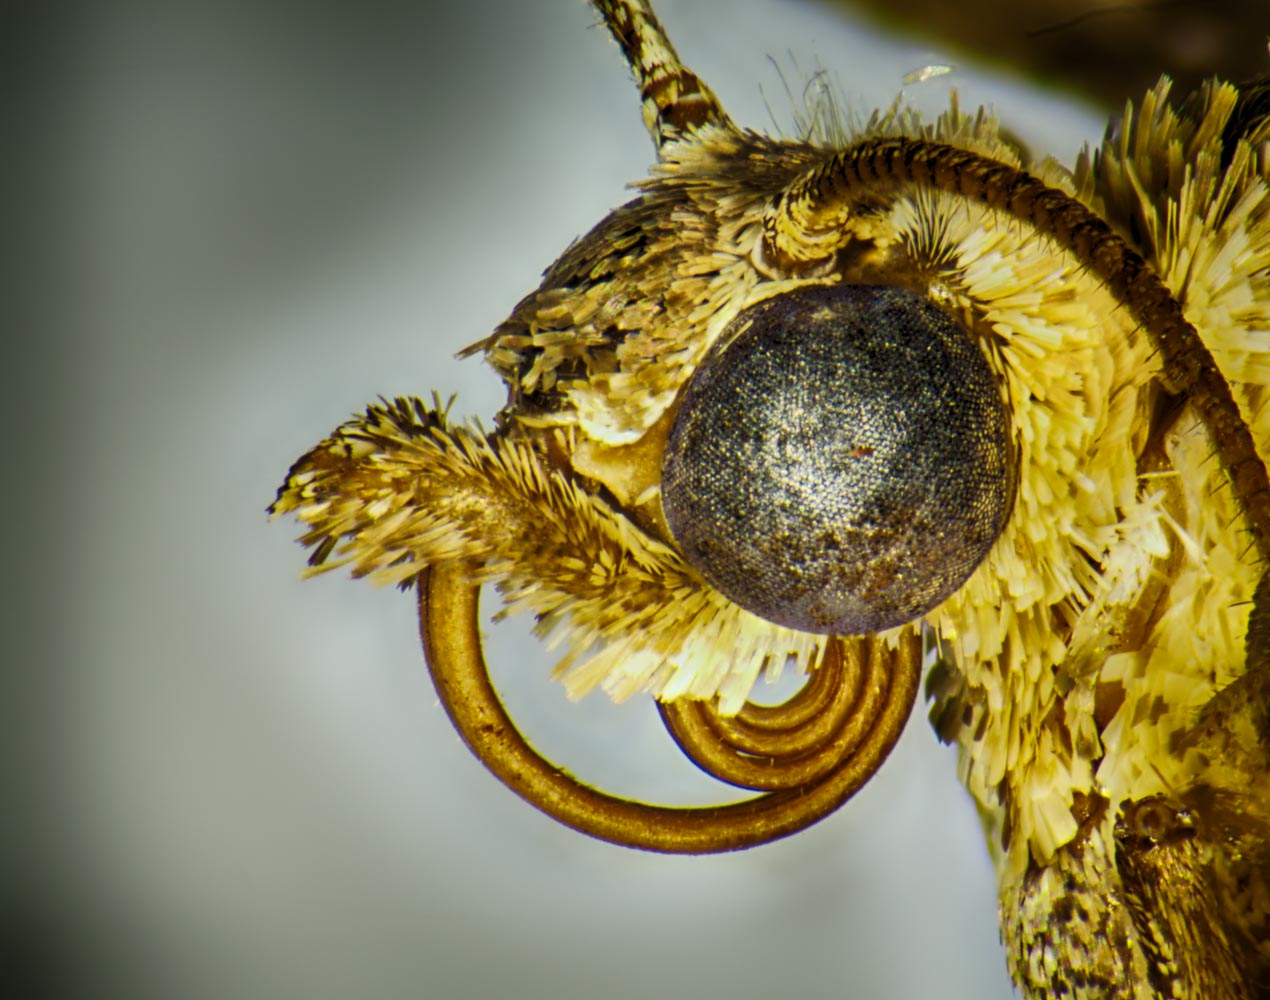
\includegraphics[width=0.5\linewidth]{images/20201112-1}
%	\caption{Short undamaged palps eliminate Hypena proboscidalis as a candidate taxon.}
%	\label{fig:20201112-1}
%\end{figure}


\bibliography{library}
\end{document}
